\documentclass[10pt,twocolumn]{article}

\usepackage[letterpaper,top=0.68in,bottom=0.72in,left=0.69in,right=0.69in,columnsep=0.25in]{geometry}
\usepackage[T1]{fontenc}
\usepackage{amsmath,mathtools,amsthm}
\usepackage{newtxtext,newtxmath}
\usepackage{microtype}
\usepackage{bm}
\usepackage{booktabs,tabularx,array,multirow}
\usepackage{enumitem}
\usepackage{graphicx}
\usepackage{xcolor}
\usepackage{tikz}
\usetikzlibrary{arrows.meta,positioning,calc,fit,backgrounds,decorations.pathreplacing,shapes.geometric}
\usepackage{algorithm}
\usepackage[noend]{algpseudocode}
\usepackage[most]{tcolorbox}
\usepackage[numbers,sort&compress]{natbib}
\usepackage{hyperref}
\usepackage[nameinlink,capitalize,noabbrev]{cleveref}
\usepackage{balance}
\usepackage{titlesec}
\usepackage{caption}

\definecolor{deepblue}{HTML}{234E70}
\definecolor{teal}{HTML}{2A7F9E}
\definecolor{orange}{HTML}{D97732}
\definecolor{green}{HTML}{4D8B55}
\definecolor{purple}{HTML}{7656A5}
\definecolor{lightblue}{HTML}{EDF5FA}
\definecolor{lightorange}{HTML}{FFF2E8}
\definecolor{lightgray}{HTML}{F3F4F6}
\definecolor{darkgray}{HTML}{3F4650}

\hypersetup{
  colorlinks=true,
  linkcolor=deepblue,
  citecolor=deepblue,
  urlcolor=teal,
  pdfauthor={Technical note},
  pdftitle={Riemannian Midpoint Generative Models}
}

\titleformat{\section}{\large\bfseries\color{deepblue}}{\thesection}{0.45em}{}
\titleformat{\subsection}{\normalsize\bfseries\color{darkgray}}{\thesubsection}{0.4em}{}
\titlespacing*{\section}{0pt}{1.0ex plus .2ex minus .2ex}{0.45ex}
\titlespacing*{\subsection}{0pt}{0.8ex plus .2ex minus .2ex}{0.25ex}
\setlength{\parindent}{1em}
\setlength{\parskip}{0pt}
\setlist[itemize]{leftmargin=1.25em,itemsep=0.15ex,topsep=0.3ex}
\captionsetup{font=small,labelfont=bf,skip=3pt}
\setlength{\textfloatsep}{7pt plus 2pt minus 2pt}
\setlength{\floatsep}{6pt plus 2pt minus 2pt}
\setlength{\intextsep}{6pt plus 2pt minus 2pt}

\newtheorem{proposition}{Proposition}
\newtheorem{corollary}{Corollary}
\newtheorem{definition}{Definition}
\newtheorem{remark}{Remark}

\newcommand{\M}{\mathcal{M}}
\newcommand{\TM}{T\!\mathcal{M}}
\newcommand{\R}{\mathbb{R}}
\newcommand{\E}{\mathbb{E}}
\newcommand{\Exp}{\operatorname{Exp}}
\newcommand{\Log}{\operatorname{Log}}
\newcommand{\Law}{\operatorname{Law}}
\newcommand{\Tr}{\operatorname{tr}}
\newcommand{\Sym}{\operatorname{Sym}}
\newcommand{\Proj}{\operatorname{Proj}}
\newcommand{\Ber}{\operatorname{Bernoulli}}
\newcommand{\Normal}{\mathcal{N}}
\newcommand{\ip}[3][]{\left\langle #2,#3\right\rangle_{#1}}
\newcommand{\norm}[2][]{\left\lVert #2\right\rVert_{#1}}
\newcommand{\dd}{\,\mathrm{d}}
\newcommand{\RMGM}{\textsc{R-MGM}}

\newtcolorbox{abstractbox}{
  colback=lightgray,
  colframe=darkgray,
  boxrule=0.45pt,
  arc=1.5pt,
  left=7pt,right=7pt,top=5pt,bottom=5pt
}
\newtcolorbox{takeaway}{
  colback=lightblue,
  colframe=deepblue,
  boxrule=0.65pt,
  arc=1.5pt,
  left=5pt,right=5pt,top=4pt,bottom=4pt,
  fonttitle=\bfseries,
  title=Main takeaway
}
\newtcolorbox{statusbox}{
  colback=lightorange,
  colframe=orange,
  boxrule=0.65pt,
  arc=1.5pt,
  left=5pt,right=5pt,top=4pt,bottom=4pt,
  fonttitle=\bfseries,
  title=Status of the theory
}

\begin{document}

\twocolumn[
\begin{@twocolumnfalse}
\vspace*{-0.35in}
{\centering
{\LARGE\bfseries Riemannian Midpoint Generative Models\par}
\vspace{3pt}
{\large A compact geometric construction for one-step generation on manifolds\par}
\vspace{6pt}
{\normalsize Technical note \textbullet\ July 2026\par}
\vspace{5pt}
{\small Based on \emph{Flow Matching on General Geometries} and \emph{Midpoint Generative Models}.\\
This document proposes an extension; it is not an official revision of either cited work.\par}
}
\vspace{8pt}
\begin{abstractbox}
\textbf{Abstract.}
Flow Matching learns a conditional velocity field, Riemannian Flow Matching (RFM) replaces straight paths and Euclidean vectors by manifold paths and tangent vectors, and Midpoint Generative Models (MGM) use a hidden endpoint flip to turn a symmetric interpolant into a discrepancy for direct one-step generator training. We combine these ideas. A reversible path selector $\Gamma(x_0,x_1,s)$ yields an observation $\widetilde X_t$ on the manifold and an orientation-odd tangent target $A_t\in T_{\widetilde X_t}\M$. The resulting conditional tangent field vanishes whenever the endpoint distributions coincide, and its squared Riemannian norm has the same fiberwise variational representation that underlies MGM. This gives a practical minimax algorithm with a manifold-valued generator and a tangent-valued critic. The transfer is exact at the level of symmetry and optimization, but not automatically at the level of definiteness: on a general curved manifold, ``zero discrepancy implies equal distributions'' requires an additional identifiability argument. We state two settings where definiteness is retained---globally Euclidean-isometric geometries, including log-Euclidean SPD matrices, and an extrinsic variant with an injective ambient embedding---and give implementation recipes for spheres, $\mathrm{SO}(3)$, SPD matrices, and general embedded manifolds.
\end{abstractbox}
\vspace{4pt}
\end{@twocolumnfalse}
]

\section{Motivation and background}

Flow Matching (FM) constructs a path of distributions from a source law $p_0$ to a target law $p_1$ and learns the vector field that transports the path without likelihood training \citep{lipman2023flow,albergo2023building}. For independent endpoints $X_0\sim p_0$ and $X_1\sim p_1$, the linear interpolant
\begin{equation}
X_t=(1-t)X_0+tX_1
\end{equation}
has conditional velocity
\begin{equation}
 v_t^\star(x)=\E[X_1-X_0\mid X_t=x].
 \label{eq:euclidean-fm}
\end{equation}
A network is trained by regressing onto the sample displacement $X_1-X_0$.

RFM extends this construction to a complete connected Riemannian manifold $(\M,g)$ \citep{chen2024general}. For a selected smooth path $\gamma_{x_0,x_1}:[0,1]\to\M$, the sample target is its tangent velocity
\begin{equation}
 a_t=\dot\gamma_{x_0,x_1}(t)\in T_{\gamma(t)}\M,
 \qquad
 v_t^\star(x)=\E[a_t\mid \gamma(t)=x],
 \label{eq:rfm-field}
\end{equation}
and tangent vectors are compared using $g_x$. On simple geometries the canonical path is the minimizing geodesic
\begin{equation}
 \gamma_{x_0,x_1}(t)=\Exp_{x_0}\!\bigl(t\Log_{x_0}(x_1)\bigr),
 \label{eq:geodesic}
\end{equation}
which is closed form on spheres, hyperbolic spaces, tori, several Lie groups, and standard SPD geometries. RFM also allows more general premetric-induced conditional flows; those paths need not be reversible, a distinction that becomes essential below.

MGM starts from a symmetry of \cref{eq:euclidean-fm}: if $p_0=p_1$, then the midpoint field vanishes. The full method uses $t\in[0,1/2]$ and an unobserved $B\sim\Ber(1/2)$ to choose between an interpolant at $t$ and its time reverse at $1-t$. The vector-valued critic predicts the endpoint displacement from this symmetrized observation. The corresponding generalized Midpoint Divergence is definite in Euclidean space and admits a variational minimax objective for training a one-step generator directly from data \citep{shlenskii2026midpoint}.

\begin{figure}[t]
\centering
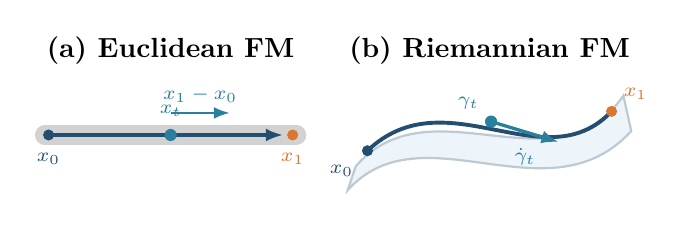
\begin{tikzpicture}[x=1cm,y=1cm,>=Latex,thick,font=\scriptsize]
  % Euclidean panel
  \node[font=\bfseries] at (1.75,1.62) {(a) Euclidean FM};
  \draw[gray!35,line width=7pt,line cap=round] (0.15,0.55)--(3.35,0.55);
  \draw[deepblue,line width=1.3pt,-{Latex[length=2.2mm]}] (0.25,0.55)--(3.18,0.55);
  \fill[deepblue] (0.2,0.55) circle (2pt) node[below=3pt] {$x_0$};
  \fill[orange] (3.3,0.55) circle (2pt) node[below=3pt] {$x_1$};
  \fill[teal] (1.75,0.55) circle (2.2pt) node[above=3pt] {$x_t$};
  \draw[teal,-{Latex[length=2mm]}] (1.75,0.83)--(2.5,0.83) node[midway,above] {$x_1-x_0$};
  % Riemannian panel
  \begin{scope}[xshift=4.05cm]
  \node[font=\bfseries] at (1.75,1.62) {(b) Riemannian FM};
  \path[fill=lightblue,draw=deepblue!30] (0.05,0.15) .. controls (1.0,1.25) and (2.6,-0.2) .. (3.45,1.05)
    -- (3.55,0.6) .. controls (2.5,-0.55) and (0.9,0.9) .. (-0.05,-0.15) -- cycle;
  \draw[deepblue,line width=1.4pt] (0.2,0.35) .. controls (1.2,1.3) and (2.45,-0.05) .. (3.3,0.85);
  \fill[deepblue] (0.2,0.35) circle (2pt) node[below left=2pt] {$x_0$};
  \fill[orange] (3.3,0.85) circle (2pt) node[above right=1pt] {$x_1$};
  \coordinate (m) at (1.77,0.72);
  \fill[teal] (m) circle (2.2pt) node[above left=1pt] {$\gamma_t$};
  \draw[teal,line width=1.2pt,-{Latex[length=2.2mm]}] (m)--++(0.86,-0.26) node[midway,below=2pt] {$\dot\gamma_t$};
  \end{scope}
\end{tikzpicture}
\caption{RFM replaces a straight interpolation and a global displacement by a manifold path and a tangent velocity.}
\label{fig:fm-rfm}
\end{figure}

\section{Intrinsic Riemannian midpoint construction}

\subsection{Reversible paths and the hidden flip}

The essential MGM ingredient is not linearity, but reversal symmetry.

\begin{definition}[Reversible tangent interpolant]
A path selector $\Gamma$ assigns a differentiable curve $\gamma_{x_0,x_1}(s)=\Gamma(x_0,x_1,s)$ with $\gamma(0)=x_0$, $\gamma(1)=x_1$, and
\begin{equation}
 \gamma_{x_1,x_0}(s)=\gamma_{x_0,x_1}(1-s).
 \label{eq:reversible}
\end{equation}
Consequently,
$\dot\gamma_{x_1,x_0}(s)=-\dot\gamma_{x_0,x_1}(1-s)$.
\end{definition}

For unique minimizing geodesics, \cref{eq:geodesic} satisfies \cref{eq:reversible}. If minimizing geodesics are not unique, the selection rule itself must be measurable and reversible. A practical numerical rule is to compute one path for the unordered endpoint pair and obtain the opposite orientation by reversing the stored path, rather than solving twice.

Let $t\sim\mathcal U[0,1/2]$, $B\sim\Ber(1/2)$, and set
\begin{equation}
 S_t=t+B(1-2t)\in\{t,1-t\}.
\end{equation}
Given $X_0\sim p_0$ and $X_1\sim p_1$, define
\begin{equation}
 \widetilde X_t=\gamma_{X_0,X_1}(S_t),\qquad
 A_t=\dot\gamma_{X_0,X_1}(S_t)\in T_{\widetilde X_t}\M.
 \label{eq:flipped-rm}
\end{equation}
The flip $B$ is hidden from the critic. The conditional tangent field is
\begin{equation}
 \widetilde v_t(x)=\E[A_t\mid \widetilde X_t=x]\in T_x\M.
 \label{eq:conditional-tangent}
\end{equation}
Conditional expectation is taken fiberwise: once $\widetilde X_t=x$ is fixed, all target vectors lie in the same Hilbert space $(T_x\M,g_x)$.

\begin{proposition}[Flip-induced cancellation]
Assume \cref{eq:reversible}, square-integrable path velocities, and $X_0,X_1\stackrel{\mathrm{iid}}{\sim}p$. Then, for every $t\in[0,1/2]$,
\begin{equation}
 \widetilde v_t(x)=0
 \quad\text{for }\Law(\widetilde X_t)\text{-almost every }x.
 \label{eq:cancellation}
\end{equation}
\end{proposition}

\noindent\textit{Proof sketch.}
The transformation $(X_0,X_1,B)\mapsto(X_1,X_0,1-B)$ preserves the joint law. By \cref{eq:reversible}, it leaves $\widetilde X_t$ unchanged and sends $A_t$ to $-A_t$. Hence the conditional law of $A_t$ given $\widetilde X_t$ is centrally symmetric.

This motivates the intrinsic Riemannian midpoint discrepancy
\begin{equation}
 \mathcal D_{\Gamma}^{\M}(p_0,p_1)
 =\int_0^{1/2}\E\!\left[
   \norm[g_{\widetilde X_t}]{\widetilde v_t(\widetilde X_t)}^2
 \right]\dd t.
 \label{eq:rm-discrepancy}
\end{equation}
It is nonnegative and equals zero whenever $p_0=p_1$.

\begin{figure}[t]
\centering
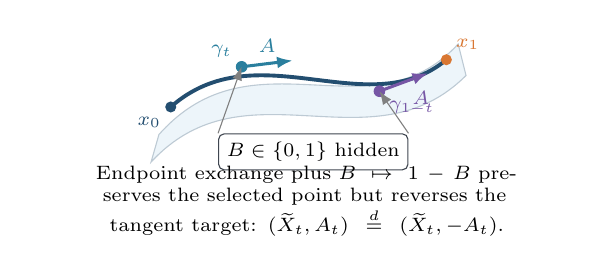
\begin{tikzpicture}[x=1cm,y=1cm,>=Latex,font=\scriptsize]
  \path[fill=lightblue,draw=deepblue!30] (-0.1,-0.2) .. controls (1.1,1.15) and (2.6,-0.25) .. (3.7,0.95)
    -- (3.8,0.55) .. controls (2.6,-0.65) and (1.0,0.75) .. (-0.2,-0.55) -- cycle;
  \draw[deepblue,line width=1.4pt] (0.05,0.15) .. controls (1.15,1.12) and (2.55,-0.08) .. (3.55,0.75);
  \fill[deepblue] (0.05,0.15) circle (2pt) node[below left] {$x_0$};
  \fill[orange] (3.55,0.75) circle (2pt) node[above right] {$x_1$};
  \coordinate (a) at (0.95,0.66);
  \coordinate (b) at (2.7,0.35);
  \fill[teal] (a) circle (2.1pt) node[above left] {$\gamma_t$};
  \fill[purple] (b) circle (2.1pt) node[below right] {$\gamma_{1-t}$};
  \draw[teal,-{Latex[length=2mm]},line width=1.1pt] (a)--++(0.65,0.08) node[midway,above] {$A$};
  \draw[purple,-{Latex[length=2mm]},line width=1.1pt] (b)--++(0.62,0.23) node[midway,below right=-1pt] {$A$};
  \node[draw=darkgray,rounded corners=2pt,fill=white,inner sep=3pt] (flip) at (1.86,-0.42) {$B\in\{0,1\}$ hidden};
  \draw[-{Latex[length=1.7mm]},gray] (flip.north west)--(a);
  \draw[-{Latex[length=1.7mm]},gray] (flip.north east)--(b);
  \node[align=center,text width=6.8cm] at (1.75,-1.05) {Endpoint exchange plus $B\mapsto1-B$ preserves the selected point but reverses the tangent target: $(\widetilde X_t,A_t)\stackrel d=(\widetilde X_t,-A_t)$.};
\end{tikzpicture}
\caption{The hidden flip removes orientation bias at every sampled time, not only at the midpoint.}
\label{fig:hidden-flip}
\end{figure}

\subsection{Variational objective and one-step training}

The Hilbert-space identity used by MGM applies independently in each tangent fiber.

\begin{proposition}[Fiberwise variational form]
For fixed endpoint laws and any square-integrable tangent field $A_t$ in \cref{eq:flipped-rm},
\begin{align}
\mathcal D_{\Gamma}^{\M}(p_0,p_1)
=\sup_f\int_0^{1/2}\E\bigl[&2g_{\widetilde X_t}(f_t(\widetilde X_t),A_t)\notag\\[-2pt]
&-\norm[g_{\widetilde X_t}]{f_t(\widetilde X_t)}^2\bigr]\dd t,
\label{eq:variational}
\end{align}
where $f_t(x)\in T_x\M$. The maximizer is $f_t^\star(x)=\widetilde v_t(x)$.
\end{proposition}

\noindent\textit{Proof sketch.}
Condition on $\widetilde X_t=x$ and complete the square in $(T_x\M,g_x)$. No global vector-space structure is needed.

Let $X_0=G_\theta(Z)$ be the one-step generator output and $X_1\sim p_{\mathrm{data}}$. Parameterizing $f$ by a tangent-valued network $f_\psi$ gives
\begin{align}
 \min_\theta\max_\psi\ \mathcal L_{\RMGM}(\theta,\psi)
 =\E\bigl[&2g_{\widetilde X_t}(f_\psi(t,\widetilde X_t),A_t)\notag\\[-2pt]
 &-\norm[g_{\widetilde X_t}]{f_\psi(t,\widetilde X_t)}^2\bigr],
 \label{eq:minmax}
\end{align}
up to the constant normalization induced by sampling $t$ uniformly. As in MGM, the critic is most conveniently updated by tangent regression,
\begin{equation}
 \mathcal L_{\mathrm{crit}}
 =\E\norm[g_{\widetilde X_t}]{f_\psi(t,\widetilde X_t)-A_t}^2,
 \label{eq:critic-loss}
\end{equation}
whereas the generator minimizes the integrand of \cref{eq:minmax} with $\psi$ frozen. The generator gradient must pass through the manifold constraint, the path solver, the target velocity, and the position-dependent metric.

\begin{algorithm}[t]
\caption{Intrinsic Riemannian MGM}
\label{alg:rmgm}
\begin{algorithmic}[1]
\Require $G_\theta: \mathcal Z\to\M$, tangent critic $f_\psi$, reversible path selector $\Gamma$
\Repeat
  \State Sample $z$ and $x_1\sim p_{\mathrm{data}}$
  \State Sample $t\sim\mathcal U[0,1/2]$ and $B\sim\Ber(1/2)$
  \State $x_0\gets G_\theta(z)$; $s\gets t+B(1-2t)$
  \State $\widetilde x\gets\Gamma(x_0,x_1,s)$; $a\gets\partial_s\Gamma(x_0,x_1,s)$
  \State Update $\psi$ by descending $\norm[g_{\widetilde x}]{f_\psi(t,\widetilde x)-a}^2$ (detach $\theta$)
  \State Resample a fresh batch and recompute $(\widetilde x,a)$
  \State Update $\theta$ by descending $2g_{\widetilde x}(f_\psi,a)-\norm[g_{\widetilde x}]{f_\psi}^2$ (freeze $\psi$)
\Until{convergence}
\State \Return $G_\theta$
\end{algorithmic}
\end{algorithm}

\begin{figure*}[t]
\centering
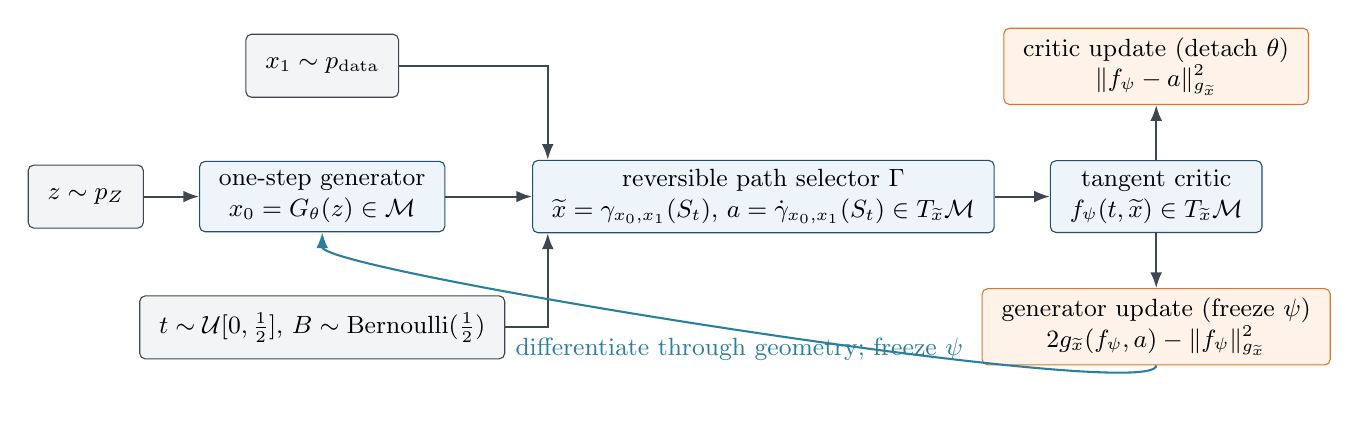
\begin{tikzpicture}[>=Latex,font=\small,node distance=5mm and 7mm]
\tikzset{
  block/.style={draw=deepblue,rounded corners=2pt,fill=lightblue,minimum height=8mm,align=center,inner xsep=7pt},
  source/.style={draw=darkgray,rounded corners=2pt,fill=lightgray,minimum height=8mm,align=center,inner xsep=7pt},
  loss/.style={draw=orange,rounded corners=2pt,fill=lightorange,minimum height=8mm,align=center,inner xsep=7pt},
  arr/.style={-{Latex[length=2mm]},line width=.75pt,draw=darkgray}
}
\node[source] (z) {$z\sim p_Z$};
\node[block,right=of z] (gen) {one-step generator\\$x_0=G_\theta(z)\in\M$};
\node[source,above=8mm of gen] (data) {$x_1\sim p_{\rm data}$};
\node[source,below=8mm of gen] (flip) {$t\sim\mathcal U[0,\tfrac12]$,\ $B\sim\Ber(\tfrac12)$};
\node[block,right=11mm of gen] (path) {reversible path selector $\Gamma$\\$\widetilde x=\gamma_{x_0,x_1}(S_t)$,\ $a=\dot\gamma_{x_0,x_1}(S_t)\in T_{\widetilde x}\M$};
\node[block,right=of path] (critic) {tangent critic\\$f_\psi(t,\widetilde x)\in T_{\widetilde x}\M$};
\node[loss,above=7mm of critic] (closs) {critic update (detach $\theta$)\\$\|f_\psi-a\|_{g_{\widetilde x}}^2$};
\node[loss,below=7mm of critic] (gloss) {generator update (freeze $\psi$)\\$2g_{\widetilde x}(f_\psi,a)-\|f_\psi\|_{g_{\widetilde x}}^2$};
\draw[arr] (z)--(gen);
\draw[arr] (gen)--(path);
\draw[arr] (data.east)-|($(path.north west)+(2mm,0)$);
\draw[arr] (flip.east)-|($(path.south west)+(2mm,0)$);
\draw[arr] (path)--(critic);
\draw[arr] (critic)--(closs);
\draw[arr] (critic)--(gloss);
\draw[arr,teal] (gloss.south) .. controls +(0,-5mm) and +(0,-5mm) .. node[below,text=teal] {differentiate through geometry; freeze $\psi$} (gen.south);
\end{tikzpicture}
\caption{Computational graph for intrinsic Riemannian MGM. The critic and target meet in the same tangent fiber, while the generator gradient propagates through the manifold parameterization, path, target velocity, and metric.}
\label{fig:pipeline}
\end{figure*}

\section{What transfers exactly---and what does not}

\begin{takeaway}
Replacing the linear path by a reversible manifold path, the global displacement by an orientation-odd tangent velocity, and the Euclidean norm by $g_x$ is sufficient to transfer the MGM cancellation mechanism and its variational training objective. It is \emph{not}, by itself, sufficient to transfer the Euclidean definiteness theorem on every curved manifold.
\end{takeaway}

The easy direction is \cref{eq:cancellation}: $p_0=p_1$ implies $\mathcal D_{\Gamma}^{\M}=0$. The converse depends on whether the family of conditional tangent moments separates probability measures on the chosen geometry. The proof of Euclidean MGM exploits the globally shared displacement $X_1-X_0\in\R^d$ and endpoint limits of the symmetric interpolant \citep{shlenskii2026midpoint}; a curved manifold has no canonical subtraction of endpoints, and projecting information into tangent fibers can discard globally identifying components.

\begin{proposition}[Definiteness on globally flat coordinates]
Suppose $\Phi:(\M,g)\to(V,\langle\cdot,\cdot\rangle)$ is a global Riemannian isometry onto a Euclidean vector space, and define
\begin{equation}
 \gamma_{x_0,x_1}(t)=\Phi^{-1}\!\bigl((1-t)\Phi(x_0)+t\Phi(x_1)\bigr).
\end{equation}
Then the intrinsic discrepancy \cref{eq:rm-discrepancy} equals the Euclidean time-integrated Midpoint Divergence between $\Phi_\#p_0$ and $\Phi_\#p_1$. Under the moment assumptions of MGM, it is definite.
\end{proposition}

\begin{corollary}[Log-Euclidean SPD matrices]
For $\M=\mathbb S_{++}^n$ with the log-Euclidean metric and $\Phi(X)=\log X$, \RMGM\ reduces exactly to Euclidean MGM on the vector space $\Sym(n)$. Hence the zero set identifies the endpoint distribution.
\end{corollary}

There is also a rigorous extrinsic fallback for any injectively embedded manifold $\iota:\M\hookrightarrow\R^D$: keep the reversible manifold observation $\iota(\gamma_s)$, but let the critic predict the ambient chord $\iota(X_1)-\iota(X_0)$. This is an instance of generalized MGM with a symmetric interpolant in $\R^D$, so the original definiteness theorem applies to the pushforward laws; injectivity of $\iota$ returns equality on $\M$. The price is dependence on the embedding and loss of a purely intrinsic tangent interpretation.

\begin{statusbox}
\textbf{Exact in general:} endpoint-exchange cancellation, tangent-bundle variational representation, and the alternating minimax algorithm.\\
\textbf{Exact under additional structure:} definiteness in global Euclidean coordinates or for the extrinsic ambient-target variant.\\
\textbf{Requires new analysis:} intrinsic definiteness on curved spaces such as spheres and $\mathrm{SO}(3)$.
\end{statusbox}

A second caveat concerns the full scope of RFM. Geodesics are reversible, but a generic premetric-induced conditional flow from $x_0$ to $x_1$ need not be the reverse of the flow from $x_1$ to $x_0$ \citep{chen2024general}. Such a path cannot be inserted blindly into MGM. On meshes or manifolds with boundaries, one should use a genuinely reversible two-endpoint path, explicitly symmetrize the path construction, or verify \cref{eq:reversible} numerically.

\section{Implementation on common manifolds}

\subsection{Sphere \texorpdfstring{$\mathbb S^{d-1}$}{S(d-1)}}

For $x,y\in\mathbb S^{d-1}$ away from antipodes, let $\alpha=\arccos(x^\top y)$. Then
\begin{align}
 \Log_x(y)&=\frac{\alpha}{\sin\alpha}\bigl(y-\cos\alpha\,x\bigr),\\
 \Exp_x(v)&=\cos\norm{v}\,x+\sin\norm{v}\,\frac{v}{\norm{v}}.
\end{align}
Use $\gamma_t=\Exp_x(t\Log_x y)$. A generator can normalize an unconstrained output,
$G_\theta(z)=h_\theta(z)/\norm{h_\theta(z)}$, and an embedded tangent critic can be parameterized by
\begin{equation}
 f_\psi(x,t)=(I-xx^\top)h_\psi(x,t).
\end{equation}
The metric is the ambient dot product. Clamp dot products before $\arccos$, use stable small-angle expansions, and treat near-antipodal pairs carefully because the logarithm is ill-conditioned and the minimizing geodesic is non-unique.

\subsection{\texorpdfstring{$\mathrm{SO}(3)$}{SO(3)}}

With the standard bi-invariant metric, write $\Omega=\log(R_0^\top R_1)\in\mathfrak{so}(3)$ and
\begin{equation}
 \gamma_t=R_0\exp(t\Omega),\qquad \dot\gamma_t=\gamma_t\Omega.
\end{equation}
A particularly stable critic outputs a left-trivialized vector $\omega_\psi(R,t)\in\R^3$ and represents the tangent vector as $R[\omega_\psi]_\times$. The loss then uses an ordinary dot product in the Lie algebra. A generator may normalize a quaternion output and map it to $\mathrm{SO}(3)$, remembering that $q$ and $-q$ represent the same rotation. Select the shortest quaternion arc or the principal matrix logarithm, and handle relative angles near $\pi$, where the logarithm is multivalued.

\subsection{SPD matrices}

A Cholesky generator
\begin{equation}
 G_\theta(z)=L_\theta(z)L_\theta(z)^\top+\varepsilon I
\end{equation}
with positive diagonal entries enforces $G_\theta(z)\in\mathbb S_{++}^n$. Under the affine-invariant metric,
\begin{align}
 g_X(U,V)&=\Tr(X^{-1}UX^{-1}V),\\
 \gamma_t&=X_0^{1/2}\bigl(X_0^{-1/2}X_1X_0^{-1/2}\bigr)^tX_0^{1/2}.
\end{align}
Every symmetric matrix is tangent, so symmetrizing the network output is sufficient; whitening $U\mapsto X^{-1/2}UX^{-1/2}$ gives Frobenius coordinates for the metric. Matrix powers, logarithms, and square roots require eigendecompositions, typically $O(n^3)$ per pair, and benefit from eigenvalue floors and higher precision near singularity. RFM experiments on SPD data found both the Riemannian path and Riemannian norm important for respecting the domain \citep{chen2024general}.

For the log-Euclidean metric \citep{arsigny2006log}, use
\begin{equation}
 \gamma_t=\exp\bigl((1-t)\log X_0+t\log X_1\bigr),
\end{equation}
run the critic in symmetric log coordinates, and inherit Euclidean MGM definiteness by the corollary above.

\subsection{General embedded manifolds}

For $\M\subset\R^D$ with induced metric, an ambient network can be projected,
\begin{equation}
 f_\psi(x,t)=\Pi_{T_x\M}h_\psi(x,t).
\end{equation}
The generator may use an exact parameterization, projection, exponential map, or a retraction. A generic retraction-based path is not automatically reversible; if it is used, enforce symmetry by construction. For general geometries where closed-form geodesics are unavailable, RFM proposes premetric and spectral constructions \citep{chen2024general}; RMGM additionally requires the resulting two-endpoint path to satisfy \cref{eq:reversible}.

\begin{table}[H]
\centering
\caption{Implementation map. The last column records the main geometric failure mode.}
\label{tab:recipes}
\scriptsize
\setlength{\tabcolsep}{3.2pt}
\renewcommand{\arraystretch}{1.16}
\begin{tabularx}{\columnwidth}{@{}>{\bfseries}p{1.22cm}p{3.18cm}X@{}}
\toprule
Geometry & Native recipe & Main caveat \\
\midrule
$\mathbb S^{d-1}$ & normalize $G$; great-circle path; $(I-xx^\top)h_\psi$ & antipodes; intrinsic definiteness open \\
$\mathrm{SO}(3)$ & quaternion/Lie generator; $R_0\exp(t\log(R_0^\top R_1))$; left-trivialized critic & $q\sim-q$ and angle $\pi$ \\
SPD--AIRM & Cholesky generator; matrix-power geodesic; whitened symmetric critic & spectral cost; intrinsic definiteness open \\
SPD--logE & interpolate and train in $\log X\in\Sym(n)$ & globally flat; definiteness transfers \\
Embedded $\M$ & reversible path; $\Pi_{T_x\M}h_\psi$ & generic retractions need not reverse \\
\bottomrule
\end{tabularx}
\end{table}

\section{Stochastic interpolants and numerical nuances}

The deterministic construction is the cleanest starting point, but the MGM experiments report substantially better Euclidean image training with mild interpolant noise and time integration \citep{shlenskii2026midpoint}. An intrinsic noisy analogue can be built from the clean point $\bar X_t=\gamma(S_t)$:
\begin{align}
 \xi_t&\sim\Normal(0,I_{T_{\bar X_t}\M}),\qquad
 X_t^\sigma=\Exp_{\bar X_t}(\sigma_t\xi_t),\notag\\
 A_t^\sigma&=\mathsf P_{\bar X_t\to X_t^\sigma}A_t.
 \label{eq:noisy}
\end{align}
where $\mathsf P$ is parallel transport along the short noise geodesic and $\sigma_t=\sigma_{1-t}$ with vanishing endpoint noise. A heat-kernel perturbation is more intrinsic but typically more expensive. Small $\sigma_t$ avoids ambiguity in the noise logarithm and reduces curvature distortion.

Three implementation details matter disproportionately:
\begin{itemize}
 \item \textbf{Differentiate through geometry.} The generator update depends on $x_0$ through $\gamma$, $A_t$, $f_\psi(t,\widetilde X_t)$, and possibly $g_{\widetilde X_t}$. Stopping gradients through the target changes the objective.
 \item \textbf{Preserve reversal numerically.} Independent forward and backward geodesic solves can differ. Reuse one discrete path in reverse, including the same discretization and branch choices.
 \item \textbf{Control the cut locus.} Reject, regularize, or consistently branch pairs for which $\Log$ is unstable. Exact antipodes or angle-$\pi$ rotations are not merely numerical edge cases: they destroy uniqueness of the midpoint.
\end{itemize}

\subsection{Minimal validation protocol}
Before large-scale training, four small tests can separate geometric bugs from optimization failures. First, draw both endpoints from the same empirical distribution and verify that the fitted conditional field norm approaches zero. Second, measure a \emph{reversal residual},
\begin{equation}
 r_{\rm rev}=d\!\left(\gamma_{x_1,x_0}(s),\gamma_{x_0,x_1}(1-s)\right)
 +\norm{\dot\gamma_{x_1,x_0}(s)+\dot\gamma_{x_0,x_1}(1-s)},
\end{equation}
using a common tangent representation for the velocity comparison; it should be at numerical precision away from the cut locus. Third, compare the critic-regression optimum with the value of the variational objective on a frozen generator. Finally, on SPD data, compare affine-invariant, log-Euclidean, and ambient-target variants: this isolates the effect of geometry from the effect of a known definiteness guarantee.

\section{Discussion}

The natural manifold extension of MGM is therefore more precise than the slogan ``replace FM by RFM.'' One must retain the hidden flip, use a reversible two-endpoint path, express the orientation signal in the tangent space of the selected observation, and train with the local Riemannian metric. With those changes, midpoint cancellation and the variational critic objective transfer cleanly, yielding a practical one-step manifold generator.

The main unresolved theoretical question is intrinsic identifiability on curved manifolds. Establishing it for spheres, compact Lie groups, Hadamard manifolds, or specific quotient geometries would turn the discrepancy in \cref{eq:rm-discrepancy} into a genuine divergence for those classes. Until such a theorem is available, the intrinsic method should be described as a symmetry-calibrated discrepancy, while the log-Euclidean and extrinsic constructions provide settings with a direct definiteness guarantee.

\bibliographystyle{unsrtnat}
\bibliography{references}

\end{document}
